%\documentclass[tikz, margin=3mm]{standalone}
\documentclass{article}
\usepackage{tikz}
\usetikzlibrary{matrix}
\newcommand\x{\times}

\begin{document}
%%% step0_cover
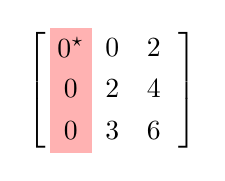
\begin{tikzpicture}
\matrix [matrix of math nodes,
         nodes={rectangle,
                minimum size=1.5em, text depth=0.25ex,
                inner sep=0pt, outer sep=0pt,
                anchor=center},
         %row 2/.append style = {nodes={preaction={fill=cyan!30}}},
         column 1/.append style = {nodes={fill=red!60},fill opacity=0.5, text opacity=1},
         inner sep=0pt,
         left delimiter={[}, right delimiter={]},
         ]
{
0^\star & 0  & 2 \\
0 & 2  & 4 \\
0 & 3  & 6 \\
};
\end{tikzpicture}

%%% step1_prime
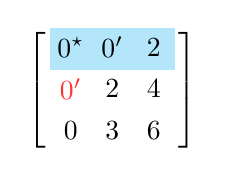
\begin{tikzpicture}
\matrix [matrix of math nodes,
         nodes={rectangle,
                minimum size=1.5em, text depth=0.25ex,
                inner sep=0pt, outer sep=0pt,
                anchor=center},
         row 1/.append style = {nodes={preaction={fill=cyan!30}}},
         %column 1/.append style = {nodes={fill=red!60},fill opacity=0.5, text opacity=1},
         inner sep=0pt,
         left delimiter={[}, right delimiter={]},
         ]
{
0^\star & 0^\prime  & 2 \\
|[text=red!80]|0^\prime & 2  & 4 \\
0 & 3  & 6 \\
};
\end{tikzpicture}

%%% step2_cover
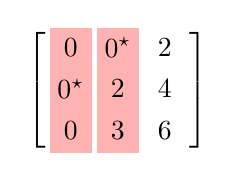
\begin{tikzpicture}
\matrix [matrix of math nodes,
         column sep = 2pt,
         nodes={rectangle,
                minimum size=1.5em, text depth=0.25ex,
                inner sep=0pt, outer sep=0pt,
                anchor=center},
         %row 1/.append style = {nodes={preaction={fill=cyan!30}}},
         column 1/.append style = {nodes={fill=red!60},fill opacity=0.5, text opacity=1},
         column 2/.append style = {nodes={fill=red!60},fill opacity=0.5, text opacity=1},
         inner sep=0pt,
         left delimiter={[}, right delimiter={]},
         ]
{
0 & 0^\star  & 2 \\
0^\star & 2  & 4 \\
0 & 3  & 6 \\
};
\end{tikzpicture}

%%% step3_min
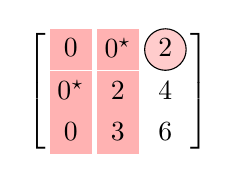
\begin{tikzpicture}
\matrix [matrix of math nodes,
         column sep = 2pt,
         nodes={rectangle,
                minimum size=1.5em, text depth=0.25ex,
                inner sep=0pt, outer sep=0pt,
                anchor=center},
         %row 1/.append style = {nodes={preaction={fill=cyan!30}}},
         column 1/.append style = {nodes={fill=red!60},fill opacity=0.5, text opacity=1},
         column 2/.append style = {nodes={fill=red!60},fill opacity=0.5, text opacity=1},
         inner sep=0pt,
         left delimiter={[}, right delimiter={]},
         ]
{
    0 & 0^\star  & |[draw, circle, fill=red!20]|2 \\
0^\star & 2  & 4 \\
0 & 3  & 6 \\
};
\end{tikzpicture}
\end{document}
